\documentclass[12 pt, a4paper]{report}
\usepackage{setspace}
\usepackage{amsmath}
\usepackage[utf8]{inputenc}
\usepackage{float}
\usepackage{geometry}
\usepackage[french]{babel}
\usepackage[T1]{fontenc}
\usepackage{graphicx}
\usepackage{array}
\usepackage{verbatim}
\usepackage{fancyhdr}
\usepackage{multicol}
\usepackage{enumitem}
\usepackage{caption}
\usepackage{subcaption}
\setcounter{secnumdepth}{3}
\renewcommand\thesubsubsection{\parindent15pt}
\usepackage[dvipsnames]{xcolor}
\usepackage[colorlinks]{hyperref}
\graphicspath{ {figures/} }
\hypersetup{
	colorlinks=true,
	linktoc=all,
	linkcolor = Maroon}
\pagestyle{fancy}
\title{\begin{large} Rapport de projet 1A : groupe 38 \end{large}\\ [3ex]
\begin{Large}
	\textbf{Photographie Schlieren et onde de choc}
\end{Large}}
\author{Hovanes BOKSYAN \\
		Aymeric FREREJEAN \\
		Nada KOUDDANE \\
		Léo LAFFAY \\
		Alexandre OCKIER \\
		Yvonne SAUTRIOT \\
		Nino VIVIAND}
\newcommand{\tutor}{\textbf{Tuteur du projet :} David RIASSETTO}
\newcommand{\HRule}{\rule{\linewidth}{0.2mm}}

\begin{document}
	\begin{spacing}{1.15}
		\makeatletter
			\begin{titlepage}
				
\includegraphics[scale = 0.5]{logo.jpeg}
				\vspace{1.5cm}
				\vfill
				\begin{center}
					\HRule \\ [2ex]
					{\@title }\\
					\HRule \\ [3ex]
					{\@author}\\ [5ex]
					{\tutor}\\[7ex]
					\textbf{Membres des Jurys:}\\
					\begin{multicols}{2}
						Daniel BELLET\\
						Benoit CLEYET-MAREL\\
						\columnbreak
						Nicolas RUTY\\
						Mathias VOISIN-FRADIN
					\end{multicols}
				\vfill
				\end{center}
			\raggedleft\vfill{Phelma - juin 2022}
			\end{titlepage}
		\makeatother
	\newpage
	\thispagestyle{empty}
	\addtocounter{page}{1}
	\tableofcontents
	\newpage
	\listoffigures
	\addcontentsline{toc}{chapter}{\normalsize\listfigurename}
	\listoftables
	\addcontentsline{toc}{chapter}{\normalsize\listtablename}
	\newpage
	\fancyhf{}
	\renewcommand{\footrulewidth}{0.4pt}
	\chead{Photographie Schlieren et onde de choc}
	\cfoot{Phelma - juin 2022}
	\rfoot{\thepage}
	\section*{Introduction}
\addcontentsline{toc}{chapter}{\normalsize{Introduction}}
\textbf{L}a visualisation des ondes de choc générées par les avions permet d’étudier leur mouvement et contribue aux recherches dans le domaine de l’aéronautique et au développement de nouveaux engins. L’observation du mouvement de l’air autour des appareils supersoniques peut être réalisée à l’aide d’un dispositif simple et efficace : le dispositif d’imagerie Schlieren. Celui-ci s’appuie sur les principes de base de transferts thermiques et d’optique géométrique,  principes utiles à tout étudiant ingénieur spécialisé en physique à Phelma. Ce projet constitue donc un moyen de mise en œuvre de connaissances théoriques pour la réalisation d’un livrable concret.
\\
\\
Cependant, l’enjeu du projet réside dans les différentes contraintes qui s’imposent à l’étudiant, notamment les contraintes budgétaires. Etant donné que le projet 1A est effectué en groupe, il nécessite un bon travail de planification, de coordination et de répartition des tâches. La deuxième difficulté majeure consiste à identifier correctement les causes d’un éventuel mauvais fonctionnement du dispositif et à proposer des pistes d’amélioration.
\\
\\
L’objectif de ce rapport est donc de présenter les différents moyens déployés afin de mener à bien ce projet, ce que soit sur le niveau technique ou organisationnel. Il présentera également une analyse détaillée des résultats obtenus, en plus des difficultés rencontrées et les améliorations effectuées.
\\
\\
Ainsi, ce document est réparti en trois parties : la première porte sur les aspects techniques du dispositif d’imagerie Schlieren et de l’onde de choc. La deuxième est, quant à elle, consacrée à tous les aspects de la gestion du projet. La troisième présente les résultats obtenus, les problèmes rencontrés et les solutions auxquels il y a eu recours afin de les résoudre. Enfin, une conclusion en guise de récapitulatif sera donnée à la fin du rapport.

	\newpage
	\renewcommand{\chaptername}{\scshape Partie}
\chapter{\normalfont \scshape Effet Schlieren}
\section{Principe du dispositif}
L'air est fluide transparent, il possède un indice de réfraction qui suit une évolution linéaire par rapport à la densité~\ref{ref:LaTeX}:
\begin{align}
	n = 1\,+\,k\,\rho
\end{align}
où $\mathnormal{n}$ est l'indice de réfraction du fluide, $\mathnormal{\rho}$ sa densité et $\mathnormal{k}$ une constante appelée constante de Gladstone-Dale. Si $\mathnormal{n_i}$ et $\mathnormal{n_r}$ sont respectivement les indices de réfraction des rayons incident et réfléchi, $\mathnormal{\theta_i}$ l'angle d'incidence et $\mathnormal{\theta_r}$ l'angle de réfraction, on peut écrire la loi de Snell-Descartes :
\begin{align}
	n_i\times\,sin(\theta_i) = n_r\times\,sin(\theta_r) 
\end{align}
En faisant varier de manière non uniforme la température ou la pression de l'air, on fait apparaître des gradients de densité, ce qui fait que l'indice de réfraction ne varie pas de la même façon partout dans le fluide. Par conséquent, les rayons lumineux sont déviés, ce qui permet d'observer l'effet Schlieren.
\subsection{Dispositif avec miroir sphérique}
\subsection{Dispositif avec lentilles convergentes}
\section{Protocole et organisation}
\subsection{Cahier des charges}
Une fois l'objectif de cette partie défini, la mise en place d'un plan d'organisation s'est avérée judicieuse pour avancer dans le projet. Pour ce faire, le diagramme de GANTT de la figure~\ref{gantt_schlieren} a été établi :
\begin{figure}[H]
	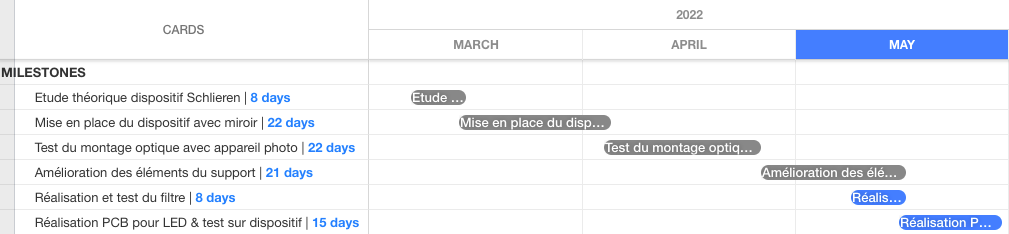
\includegraphics[scale = 0.43]{figures/gantt_schlieren.png}
	\caption{\small{\textit{Diagramme de GANTT prévu pour le montage optique}}}
	\label{gantt_schlieren}
\end{figure}
Par ailleurs, parmi les sept membres du groupe, quatre ont été chargés de mettre en place le système optique, un rôle a été attribué à chacun des membres :
\begin{table}[H]
	\centering
	\setlength{\tabcolsep}{15pt}
	\begin{tabular}{|l l l l|}
		\hline
		\vtop{\hbox{\strut \small\textbf{Chef effet}}\hbox{\strut \small\textbf{Schlieren}}}&\vtop{\hbox{\strut \small\textbf{Responsable}}\hbox{\strut \small\textbf{communication}}}&\vtop{\hbox{\strut \small\textbf{Responsable}}\hbox{\strut \small\textbf{support 3D}}}&\vtop{\hbox{\strut \small\textbf{Responsable}}\hbox{\strut \small\textbf{planning}}}\\
		\hline
		\vtop{\hbox{\strut \small{Yvonne}}\hbox{\strut \small{SAUTROIT}}}&\vtop{\hbox{\strut \small{Léo}}\hbox{\strut \small{LAFFAY}}}&\vtop{\hbox{\strut \small{Alexandre}}\hbox{\strut \small{OCKIER}}}&\vtop{\hbox{\strut \small{Nada}}\hbox{\strut \small{KOUDDANE}}}\\
		\hline
	\end{tabular}
	\caption{\small\textit{Membres et tâches attribuées (dispositif à imagerie Schlieren)}}
	\label{gestion_schlieren}
\end{table}
\subsection{Mise en place des montages optiques}
\subsubsection{\normalfont\textit{Dispositif avec miroir sphérique}}
\subsection{Améliorations des montages}
\section{Observations et conclusion}
\subsection{Description des résultats}
\subsection{Interprétation}
\subsection{Conclusion partielle}
	\newpage
	\renewcommand{\chaptername}{\scshape Partie}
\chapter{\normalfont \scshape Aspects organisationnels}
	\newpage
	\newpage
	\renewcommand{\chaptername}{\scshape Partie}
\chapter{\normalfont \scshape Photographie de l'onde de choc}
\section{Résultats attendus et limites}
D’après la relation \ref{indice_pression} (c.f. Partie 1), un autre moyen de faire varier la masse volumique du milieu est de changer la pression: c’est ce que fait une onde de choc. On fait l’hypothèse que la pression au niveau de l’onde de choc observée est la même que la pression à la rupture de la membrane (\textbf{$P$ = 2,5 bar}), ainsi en utilisant à nouveau la relation des gaz parfait on en déduit une variation d’indice optique très forte  : \\
\centerline{$\frac{\Delta n}{n}$ = \textbf{39,7 \%}}\\ \\
On s'attend donc à ce que le contraste soit bien visible dans l'image de l'onde de choc. Cependant, vu la grande variation de pression, l'onde de choc se propage à très grande vitesse. En effet, d'après la loi de \textsc{Mach} :
\begin{align}
	c= \sqrt{\gamma\,\frac{P}{\rho}}
\end{align}
Or, $\gamma = \frac{7}{5}$, ce qui donne à peu près \textbf{$c$ = 520 m/s} à \textbf{2,5 bar}.\\\\
On comprend dès à présent la difficulté qui se présente à nous : visualiser le front d’onde de l’onde de choc. Or, ce dernier se déplaçant à \textbf{520 m/s}, on peut en déduire le nombre d’images par seconde qu’il nous faut pour être certain d’en observer une : il s’agit de l’inverse du temps passé entre les 2 extrémités du miroir. On a donc $f$ la fréquence d’images (par seconde) de l’appareil photo qui doit être égale à $f = \frac{c}{d}$, $d$ étant le diamètre du miroir.
\\
\\
L’application numérique donne $f$ = \textbf{6047 ips}. Ce nombre étant largement hors de portée de la plupart des appareils, on ne peut donc pas observer le front d’onde de l’onde de choc avec certitude. On parlera donc de probabilité d’observer le front d’onde. Si la vitesse est maintenue constante, la probabilité d’observer l’onde de choc (la probabilité qu’une image soit prise au moment où l’onde de choc passe sur le miroir) est simplement le quotient du nombre d’images par seconde de l’appareil sur le nombre d’images par seconde requise pour observer avec certitude une image de l’onde de choc. Or la caméra utilisée est une caméra à \textbf{60 ips}, on en déduit donc que la probabilité d’observer le front d’onde de l’onde de choc est de $\frac{60}{6047}\,\simeq$ \textbf{1 \%}.
\section{Observations}
\begin{figure}[H]
	\centering
	
\includegraphics[scale = 0.12]{figures/choc_avant.jpg}
	\caption{\small{\textit{Image précédant l'onde de choc}}}
	\label{fig:choc_avant}
\end{figure}
\begin{figure}[H]
	\centering
	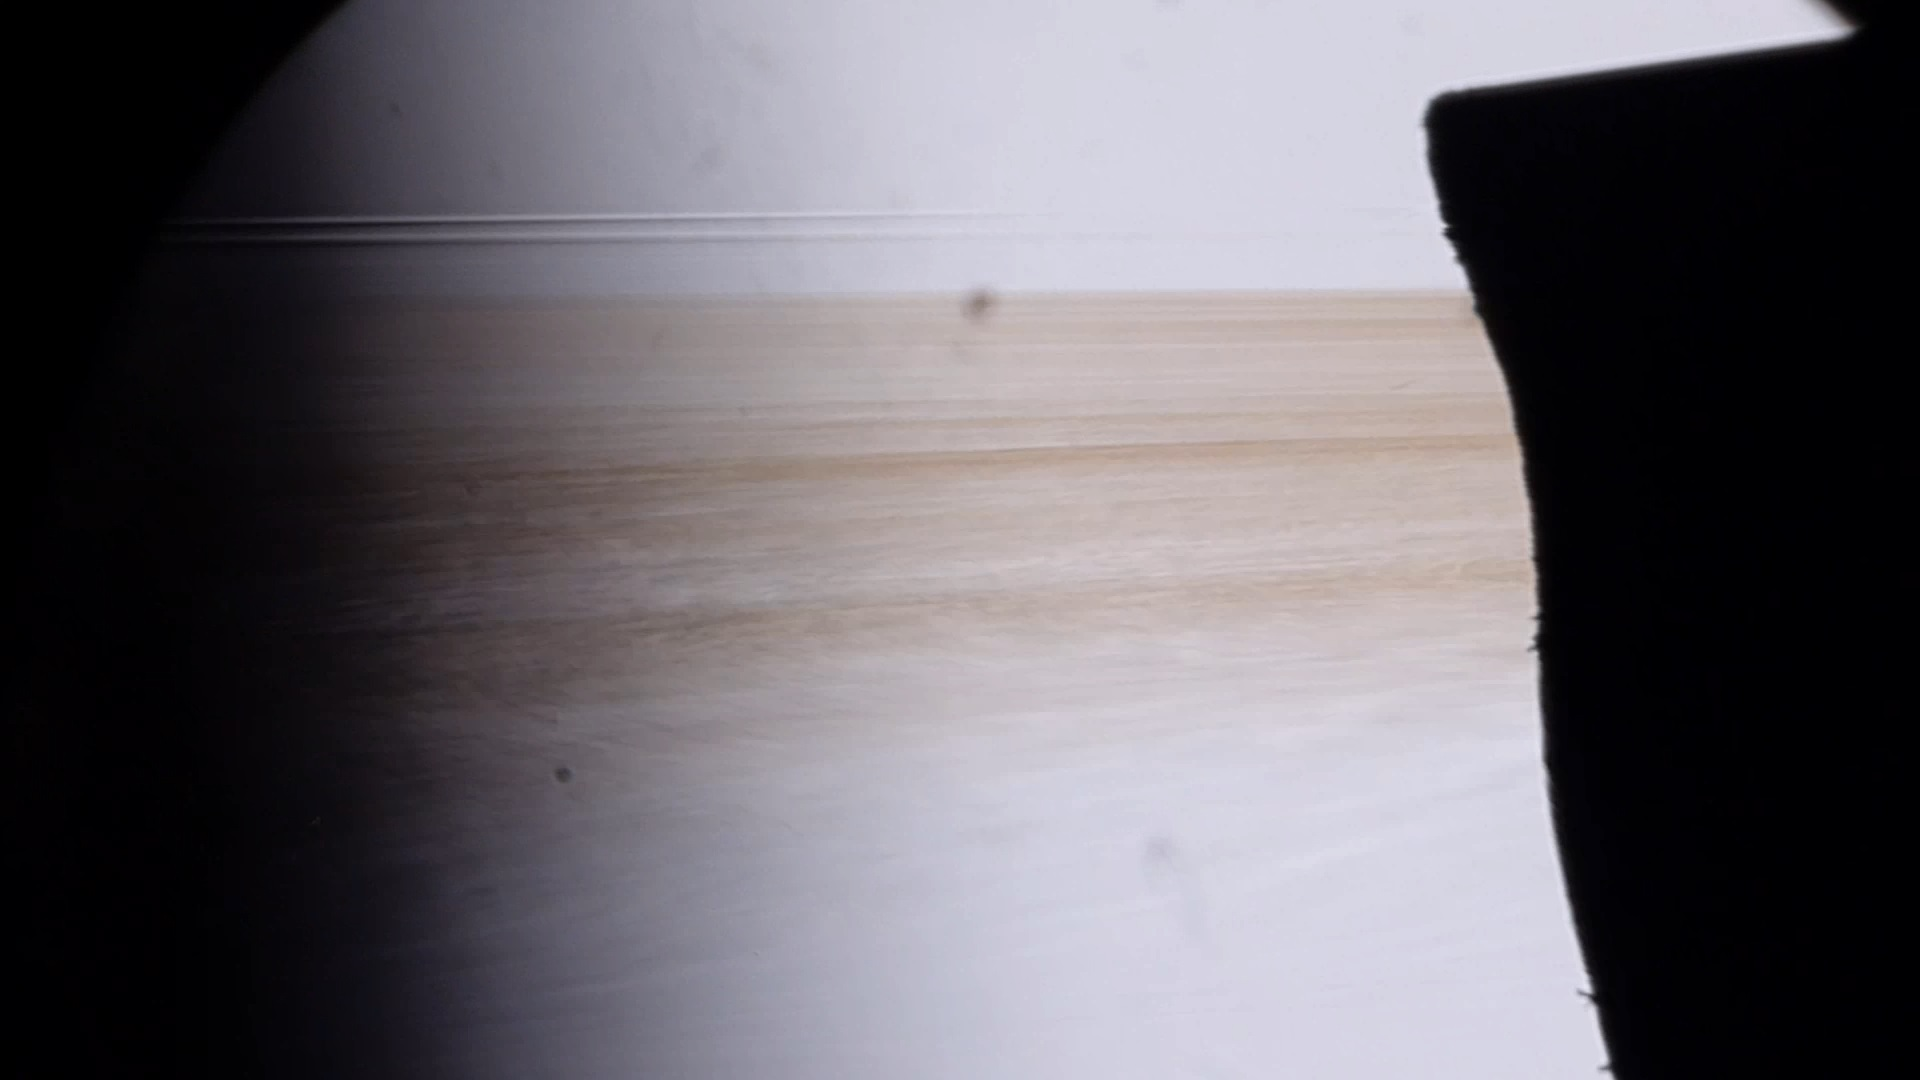
\includegraphics[scale = 0.12]{figures/choc_schlieren.jpg}
	\caption{\small{\textit{Cône de pression lié à l'onde choc, pression avant rupture : 2,5 bars}}}
	\label{fig:choc_schlieren}
\end{figure}
\begin{figure}[H]
	\centering
	
\includegraphics[scale = 0.12]{figures/choc_apres.jpg}
	\caption{\small{\textit{Image succédant l'onde de choc}}}
	\label{fig:choc_apres}
	\end{figure}
Faute de pouvoir observer le front d’onde par manque de moyens techniques on peut toutefois observer des “résidus” de l’onde de choc qui persistent plus longtemps sur la surface observable.\\\\
L’image~\ref{fig:choc_schlieren} n’est évidemment pas le front d’onde de l’onde de choc mais elle en est une conséquence directe: elle est unique donc de durée inférieure à $\frac{1}{60}$ = \textbf{17 ms} (les images la précédant (\ref{fig:choc_avant}) et la succédant (\ref{fig:choc_apres}) sont sans lien avec elle), et on observe clairement la projection de la fumée et la délimitation de pression horizontale qui en résulte.
De plus, on observe la déformation du tuyau sous l’effet de la libération de l’onde de choc.\\\\
Ces éléments permettent de conclure sur le fait que l’image observée est bien une conséquence du passage du front d’onde de l’onde de choc. Cependant, elle est difficilement observable même avec l'appareil photo disponible vu sa vitesse élevée.

	\newpage
	\section*{Références}
\addcontentsline{toc}{chapter}{\normalsize{Références}}
\parindent0pt

	\newpage
	\section*{Résumé}
\addcontentsline{toc}{chapter}{\normalsize{Résumé}}
\small{\textbf{L}a chaleur émanant d’une bougie, l’air traversant un sèche-cheveux ou encore l’onde de choc produite par un avion entraînent des fluctuations de la densité optique. Celles-ci sont toutefois invisibles à l’œil nu, il faut donc concevoir des dispositifs d’imagerie afin de pouvoir les visualiser. Ce projet a porté sur l’étude d’un système d’imagerie Schlieren, dont le principe est similaire au filtrage du son : il s’agit de couper une partie des rayons déviés par un changement d’indice de réfraction afin d’agir sur la luminosité de l’image en sortie. L’équipement consiste en un miroir sphérique, dont le but est de concentrer la lumière d’une source ponctuelle, et d’une lame de rasoir en guise de filtre. L'effet de la source de chaleur est ensuite observé à l'aide d'un appareil photo. Le système conçu a donné des résultats satisfaisants : le contraste pourrait être amélioré, mais l'effet Schlieren est bien visible. L’objectif final de ce projet est de concevoir une onde de choc et de la visualiser à l'aide du dispositif optique.}
\\
\\
\small{\textbf{Mots-clés :} effet Schlieren, onde de choc, densité optique, indice de réfraction, filtre} 

	\section*{Abstract}
\addcontentsline{toc}{chapter}{\normalsize{Abstract}}
\textbf{H}eat emanating from a candle, air coming through a hairdryer or a shock wave produced by a plane create
fluctuations in optical density. However, they aren't visible to the naked eye; a specific system is needed
in order to observe and analyse these phenomena. Schlieren imaging systems are based on light filtering:
similarly to sound filtering, the purpose is to cut off part of the incoming light to create darker spots
where it has been deflected by a change in the refractive index of the air. The device that was set in place
consists of a spherical mirror that focuses the light coming from a point source and a razor blade that acts
as a filter. Once the components are all in place, the interfering object is set in front of the mirror and the
result is captured on camera. Experiments with matches gave quite convincing results: although the
contrast and focus still need to be improved, the heat coming out was clearly visible on screen. The final
aim of this project is to generate a shockwave through a series of tubes directing air pressure and to
observe it with Schlieren photography.
\\
\\
\small{\textbf{Keywords :} Schlieren effect, shock wave, optical density, refractive index, filter}

	\end{spacing}
\end{document}